En este capítulo se presentan las principales técnicas forenses aplicadas a videos. A pesar de ser un campo ampliamente investigado, la gran cantidad de video que se produce a diario y el crecimiento de aplicaciones de edición de video para usuarios no expertos ha crecido exponencialmente en los últimos a\~nos, lo que hace que muchos de los algoritmos desarrollados queden desactualizados frente a nuevos técnicas antiforenses, que buscan no ser detectados por técnicas forenses ya existentes. 
La gran digitalización de la sociedad en las últimas décadas ha influido de forma notable en procesos judiciales, especialmente posteriormente a $1978$ puesto que tras la legislación de Florida se admitían pruebas digitales (e-mails, fotografías o videos digitales, audios, etc.) como evidencia. Para garantizar que pruebas digitales puedan considerarse como evidencia de sucesos reales tiene que garantizarse que no hayan sido manipuladas y debe poder establecerse la fuente de adquisión de los datos digitales en cuestión. \\

En las siguientes secciones se describen en detalle la detección de manipulación de videos, la detección de doble compresión (un caso concreto que permite la detección de manipulación de videos) y la identificación de la fuente. Antes, sin embargo, es necesario definir cómo se puede medir el grado de similitud entre dos imágenes, puesto que en muchas de las técnicas dentro de manipulación de videos, es necesario comparar frames o regiones de frames. \\

\section{Similitud entre fotogramas}
Detectar cuando dos frames son iguales o muy parecidos es una parte importante del análisis forense en imágenes y videos. Además de ser una herramienta muy útil en la detección de inserciones de frames en videos u objetos, también lo es para asegurar los derechos de autor. Como se explicará posteriormente, permite también obtener los frames más representativos de un video obteniendo los menos similares, técnica que permite resumir videos a través de la indexación y la navegación. En lo que sigue se exponen dos métodos ampliamente utilizados para tratar la similitud entre frames. \\

\subsection{Histogramas de color}
Este método se basa en que las imágenes o frames se corresponden con una serie de valores de píxel, e imágenes similares tendrán proporciones parecidas de ciertos colores\cite{jain:1996}. Al agrupar en clases y representar las frecuencias, el histograma no se verá afectado al manipular la orientación, tama\~no o posición de la imagen. \\

Técnicas simples como la propuesta en \cite{jain:1996} obtienen un $90\%$ de precisión para detectar imágenes similares en bases de datos. Para cada canal RGB crean un histograma y utilizan la distancia euclídea para comparar cada clase (en inglés \textit{bin}). \\

Se han desarrollado técnicas más elaboradas como la expuesta en \cite{jeong:2001} en la que utilizan un único histograma en lugar de tres, pero cada clase del histograma tiene información que relaciona todos los canales. Además, también realizan pruebas con otras variables distintas al color. Para calcular la similitud entre los histogramas, se utilizaron diferentes métodos como la distancia euclídea o la intersección de histogramas. La frecuencia además fue normalizada en base al número de pixels de cada imagen, para poder abarcar redimensionamiento de imágenes. \\

La principal desventaja que tiene el uso del histograma de color es que no tienen en cuenta características espaciales o geométricas: el mismo objeto cambiado de color no será visto como el mismo. Además, cambios en la cuantificación pueden pasar desapercibidos por algoritmos basados en el histograma de color. \\

\subsection{Perceptual hashing}
El uso de funciones \textit{hash} o funciones resumen ha sido ampliamente utilizado en criptografía. Estas funciones se han caracterizado por transformar dos entradas muy similares en salidas completamente distintas. Sin embargo, las funciones de tipo \textit{perceptual hashing} obtienen resultados muy similares para imágenes de entrada muy parecidas, de forma que la distancia entre la salida de dos \textit{perceptual hash} puede ser utilizado para comparar dos imágenes. La distancia en este caso a utilizar es la distancia de Hamming, que cuenta el número de bits que difieren.\\

Hay varios algoritmos para calcular el \textit{perceptual hash} de una imagen, aunque todos utilizan pasos similares. A continuación se describen los métodos \textit{average}, \textit{difference} y \textit{phash}. \\

El algoritmo \textit{average hash} consta de:
\begin{enumerate}
\item \textbf{Reducir el tama\~no}: se reduce la imagen a una de tama\~no $8$x$8$. De esta forma se reducen elementos de alta frecuencia y los detalles de la imagen.
\item \textbf{Reducir el color}: se convierte a escala de grises.
\item \textbf{Calcular el color medio}.
\item \textbf{Calcular el hash}: se compara cada píxel con el color medio.
\end{enumerate} 

\textit{Difference hash} sigue los mismos dos primeros pasos que \textit{average hash} pero en vez de comparar el valor del píxel con el color medio lo compara con el píxel situado a su derecha. Genera menos falsos positivos que \textit{average hash}. \\

El más complejo y más costoso computacionalmente es el algoritmo \textit{phash}:
\begin{enumerate}
\item \textbf{Reducir el tama\~no}: se reduce la imagen a una de tama\~no $32$x$32$.
\item \textbf{Obtener la luminosidad}: para cada píxel resultante se obtiene el valor de la luminosidad.
\item \textbf{Transformada DCT}: se aplica la transformada DCT a la matriz resultante del paso anterior.
\item \textbf{Bajas frecuencias}: de la matriz de $32$x$32$ obtenida en el paso anterior, se eliminan las altas frecuencias y toma únicamente los $8$x$8$ valores correspondientes con frecuencias bajas, los de más arriba y más a la izquierda.
\item \textbf{Calcular el hash}: se compara cada píxel con la mediana.
\end{enumerate}

En \cite{zhang:2017} comparan distintos métodos, entre ellos algunos basados en histogramas de color, frente a su propuesta que consisten en dos fases: en la primera extraen fotogramas en base a la entropía y en la segunda utilizan \textit{phash}, obteniendo buenos resultados. \\

\section{Manipulación de videos}
Actualmente existen multitud de herramientas de edición de video a disposición de usuarios no expertos, que pueden manipular la imagen de múltiples formas como introduciendo, quitando, repitiendo o copiando frames, además de operaciones que no a\~naden objetos al video como son la rotación, el escalado o la aplicación de filtros. En cualquiera de los dos casos, a pesar de que no haya a\~nadido o eliminado ningún objeto en frames, afectará a la codificación del video. \\

La aplicación de técnicas forenses de imágenes para la detección de manipulaciones en videos no es recomendable. La estructura de los videos y los distintos tipos de frames del GOP permiten técnicas basadas en la consistencia temporal incapaces de ser detectadas por medio de análisis estáticos de los frames considerados como imágenes, además de ser algoritmos computacionalmente costosos y de ser incapaces de detectar la inserción o eliminación de frames\cite{bestagini:2012}. \\

En \cite{chang:2013} analizan el problema de la duplicación de frames y utilizan la correlación como medida de similitud. En primer lugar eligen un conjunto de segmentos candidatos de entre todos los del video, reduciendo el espacio de búsqueda, para luego calcular la medida de similitud entre ellos a partir de histogramas de color y decidir si se ha producido duplicación o no. Para los experimentos han utilizado un conjunto de 15 videos manipulados y el algoritmo ha mostrado una precisión media del $85\%$. \\

En \cite{wu:2014} se centran en la detección de eliminación o duplicación de frames consecutivos. Para ello se basan en un término derivado de la velocidad de partículas en imágenes o PIV (del inglés \textit{Particle Image Velocity}), cuya idea es comparar frames adyacentes y estimar el desplazamiento causados por la separación en el tiempo. La duplicación o eliminación de frames consecutivos contribuye a aumentar este desplazamiento. Para decidir si un desplazamiento concreto es debido a una manipulación, utilizan el test de Grubbs\cite{wiki:grubbs} que para una distribución normal permite detectar \textit{outliers}. En los experimentos parten de $40$ videos a partir de los que generan otros $40$ eliminando frames y otros $40$ duplicando frames. La precisión media es del $96,3\%$ con una tasa de falsos positivos del $10\%$. \\

En \cite{wang:2014} se basan en que la correlación entre los coeficientes de valores grises es consistente en videos pero cuando se produce una falsificación desaparece esta consistencia. Primero extraen la consistencia de la correlación de los coeficientes de los valores grises para posteriormente clasificar las características mediante SVM (del inglés \textit{Support Vector Machine}). En los experimentos parten de una base de datos de videos originales y crean otras cuatro bases de datos a partir de los originales con las siguientes manipulaciones: insertando $25$ frames, insertando $100$ frames, eliminando $25$ frames y eliminando $100$ frames. Para entrenar la SVM utilizan $480$ videos originales y $480$ videos falsificados, dejando $118$ originales y otros tantos manipulados para pruebas, consiguiendo precisiones por encima del $90\%$. \\

Los mismos autores, en \cite{flow:2014} utilizan otro método basado también en la consistencia temporal entre frames. En este caso en lugar de utilizar la correlación entre los coeficientes grises, utilizan la consistencia medida mediante el flujo óptico de Lucas-Kanade que permite determinar el movimiento de un objeto dentro de una secuencia de frames. Para los experimentos utilizan la mismas bases de datos que en el caso anterior y una SVM para la clasificación, consiguiendo una precisión media superior también al $90\%$. \\

En \cite{kingra:2017} se basan en el flujo óptico pero lo calculan siguiendo Horn-Schunck en lugar de Lucas-Kanade. Extraen únicamente los frames tipo I y tipo P y extraen como características el PRG (del inglés \textit{Prediction Residual Gradient}) y el OFG (del inglés \textit{Optical Flow Gradient}), el primero centrado en variaciones en la posición de objetos mientras que el segundo está centrado en cambios en la luminosidad. Estas dos características son comparadas con unos umbrales determinados empíricamente para detectar picos, cuando los picos sean continuos se tratará de una manipulación. El método ha mostrado una precisión de un $86\%$ en las pruebas realizadas. \\

En \cite{jia:2018} utilizan también el flujo óptico de Lucas-Kanade para detectar inconsistencias en el caso de manipulaciones de tipo inserción o eliminación de frames. En lugar de computar la correlación entre frames del flujo óptico primero utilizan un estadístico que resume la información de los vectores resultantes de Lucas-Kanade para comprobar la consistencia con estos. Cuando se detectan irregularidades en base a este estadístico calculan la correlación entre los vectores completos del flujo Lucas-Kanade. Utilizan para las pruebas un total de $115$ videos con una precisión en torno al $90\%$. \\

Algunos autores han desarrollado métodos basados en la extracción de algún tipo de huella a partir de los frames que componen el video para detectar anomalías en frames con huellas significativamente distintas. Estos métodos tienen el incoveniente de que los videos comprimidos pierden mucha información sobre la huella, y solamente han demostrado dar buenos resultados en videos no comprimidos que suele ser poco usual. En \cite{mondaini:2007} obtienen el PRNU de los primeros frames que componen el video y utilizan distintas medidas para detectar ataques como inserción de \textit{frames}, inserción de objetos y replicación de frames mediante la correlación entre el PRNU de referencia del video y el ruido de un frame en concreto, la relación entre el ruido de dos frames consecutivos o la relación entre dos frames consecutivos. En \cite{kobayashi:2010} utilizan en lugar del PRNU un ruido que solamente es aplicable a los sensores CCD, el ruido del fotón en disparo. Además, su método solamente es aplicable a videos grabados de forma estática sin la cámara en movimiento lo cual restrige mucho el ámbito de aplicabilidad del algoritmo. En el caso en el que se den las premisas de las que parten el método tiene una precisión del $97\%$. \\

Aprovechando la consistencia entre frames de tipo temporal, algunas investigaciones se han centrado en aspectos de tipo geométrico como pueden ser que las propiedades físicas o de iluminación sean reales. En \cite{conotter:2011} se utilizan técnicas geométricas para detectar trayectorias imposibles de objetos en vuelo libre. Para ello, se modeliza el movimiento parabólico de estos objetos en tres dimensiones para proyectar este modelo posteriormente en dos dimensiones y compararlo con la trayectoria de ese mismo objeto en el video. El método desarrollado es válido tanto para cámaras estáticas como para cámaras en movimiento y se han realizado experimentos con diversos videos ya sea generados por ellos u obtenidos de plataformas de compartición de contenido en los que han medido el error medio entre la trayectoria real y la trayectoria estimada mediante su procedimiento para ser capaces de clasificar cuando una trayectoria ha sido falseada, sin embargo no hay datos sobre la precisión del algoritmo en cuestión. Hay que tener en cuenta que esta técnica solamente puede ser utilizada en videos en los que exista un objeto que describa una trayectoria parabólica y por tanto no es válida para cualquier video. \\

Sin embargo, la mayoría de trabajos sobre la detección de manipulación de videos están basados en detectar la re-comprensión o doble compresión de un video, puesto que al ser editado se vuelve a comprimir por segunda vez. 

\section{Doble compresión}
Gran parte de los estudios sobre doble compresión se centran en videos con formato MPEG y utilizan las mismas ideas que en la detección de doble compresión de imágenes JPEG. En concreto, la re-cuantificación afecta de los coeficientes DCT al usar un paso de cuantificación distinto del original, víendose en el histograma de los coeficientes DCT\cite{bestagini:2012}. Estos coeficientes pueden ser aproximados como\cite{fridrich:1998}

\begin{equation}
Y_{Q_1, Q_2} = \Delta_{2} sign(Y)round\left(\frac{\Delta_1}{\Delta_2}round\left(\frac{|Y|}{\Delta_1}\right)\right) \nonumber
\end{equation}

siendo $\Delta_1$ y $\Delta_2$ el tama\~no del paso en la primera y segunda compresión, respectivamente.

En \cite{fridrich:2003} muestran como la relación que hay entre $\Delta_1$ y $\Delta_2$ influye en el histograma creando un máximo característico. Intuitivamente, la idea es que al descomprimirse la imagen, modificarse una porción de la misma y volverse a comprimir, esa porción modificada mostrará trazas de una sola compresión mientras que el resto de la imagen tendrá rasgos de doble compresión. 

En \cite{huang:2014} presentan un método para el caso en el que se ha utilizado la misma matriz de cuantificación en ambas compresiones, basado  en el número de coeficientes DCT distintos que hay en una compresión, doble compresión y triple compresión.

En \cite{wang:2013} utilizan un conjunto de clasificadores binarios entrenados con distintas combinaciones entre $\Delta_2$ que es conocida (se puede leer directamente de los datos del video) y posibles $\Delta_1$, para luego tomar el voto de la mayoría con las características concretas del video en cuestión. \\

En \cite{tariang:2017} se basan en aplicar que se obtiene lo mismo si se comprime la imagen una vez con $\Delta_1$ que si se comprime dos veces con la misma matriz de cuantificación $\Delta_1$. De esta forma, dada la imagen original vuelven a comprimirla con distintas matrices hasta encontrar una que cumpla que en la mayoría de los bloques codificados se tenga la imagen original, obteniendo así la matriz de cuantificación que se utilizó en la última compresión. La manipulación se detecta en el caso de que existan algunos bloques distintos entre la imagen comprimida y la original, puesto que entonces la última compresión no ha sido aplicada por igual en todos los bloques y ha existido una doble compresión. Para la experimentación contaron con un conjunto de $1338$ imágenes y dentro de las pruebas que realizaron la peor precisión media que obtuvieron fue del $88,7\%$. Es importante tener en cuenta que si la imagen ha sido manipulada y se ha utilizado la misma matriz de cuantificación que en la primera compresión, este método no logrará detectarlo. \\

En \cite{sun:2013} se extraen los coeficientes DCT para luego calcular las diferencias entre ellos en cuatro direcciones: horizontal, vertical, diagonal mayor y diagonal menor. Tras obtener estas cuatro matrices se truncan algunos elementos basados en ciertos umbrales para luego ser modeladas cada uno por medio de un proceso aleatorio de Markov de primer orden. Tras algunas transformaciones sobre estos procesos de Markov, se crea un array de características que será tratado por algoritmos de \textit{machine learning} puesto que la doble compresión conlleva unos errores de redondeo que dejan muestras estadísticas caracterizables por Markov. Para la experimentación generan $5040$ videos con la misma estructura GOP y con distintas combinaciones $\Delta_1$ y $\Delta_2$, con una precisión superior al $90\%$. \\

Otra estrategia ampliamente utilizada se basa en que mientras que los coeficientes DCT de una imagen siguen una distribución Laplace\cite{reininger:1983} o una distribución Cauchy\cite{eggerton:1986}, también siguen la ley de Benford\cite{fu:2009}, esto es, el primer dígito significativo es $d$ con probabilidad $\log_{10}\left(1+\frac{1}{d}\right)$. Si los coeficientes DCT se alejan significativamente de esta distribución entonces podemos concluir que se ha utilizado doble compresión. Muchas investigaciones han utilizado procedimientos basados en la ley de Benford aplicados al caso de doble compresión JPEG en imágenes, extensibles al caso de video. 

En \cite{wang:2009} parten de la hipótesis que el factor de multiplicación $q_1$ de la tabla de cuantificación y el factor $q_2$ de la segunda tabla de cuantificación varían mientras que la tabla se mantiene la misma. En el caso de que $q_1 > q_2$ se observan anomalías en el histograma de los coeficientes DCT de tipo AC (frecuencia distinta de cero en ambas dimensiones espaciales) distintos de cero y es posible detectar la doble compresión. \\

En \cite{milani:2012} aplican la ley de Benford para un subconjunto de las frecuencias del DCT que identifican más sensible al número de compresiones y utilizan un multiclasificador compuesto de $N$ clasificadores SVM $S_k (k=1, \dots, N)$ donde $S_k$ es un clasificador binario que detecta si la imagen ha sido comprimida $k$ veces o no. De esta forma el número de compresiones que ha sufrido la imagen se toma como el clasificador con mayor $k$ que haya detectado que ha sido comprimido $k$ veces. Para la experimentación se ha trabajado con un conjunto de prueba de $100$ imágenes y un conjunto de test de $10$ imágenes, donde han obtenido una precisión del $94\%$ considerando que como máximo podía haber $N=4$ compresiones.

En \cite{chen:2009} aplican la ley de Benford para videos puesto que la codificación MPEG para videos y JPEG para imágenes comparten el mismo proceso. Observan que cuando se utiliza VBR los coeficientes AC distintos de cero de los I-frames doblemente comprimidos se alejan de la ley de Benford solamente cuando la escala de cuantificación utilizada en $\Delta_2$ es menor que la utilizada en $\Delta_1$. En el caso de CBR sí que aprecian compartamientos anómalos sin distinción de casuística. Para formalizar lo anterior, utilizan clasificadores binarios SVM en los que tratan como unidad un GOP decidiendo que existe doble compresión si el porcentaje de frames detectados como doblemente comprimidos excede un umbral determinado, obteniendo una precisión media superior al $95\%$. \\

Los métodos descritos arriba se basan en extender técnicas desarrolladas para imágenes para el caso de video. Sin embargo, existen otros algoritmos que aprovechan la alteración de la estructura GOP de los videos. Dentro de un GOP, los P-frames están correlacionados con el I-frame inicial, de forma que en caso de existir doble compresión los frames que cambien de GOP, ver figura \ref{fig_doble-compresion} mostrarán ciertas características estadísticas.

En \cite{farid:2009} se centran en el error de movimiento o compensación de movimiento de los P-frames, esto es, la transformación que se debe aplicar a un frame de tipo I o de tipo P anterior para obtener el P-frame en cuestión. Al deshacerse la secuencia original GOP, existirán P-frames cuyo frame de referencia haya cambiado y el error de movimiento en ese caso es mayor. En este trabajo no se describe el método para determinar el umbral que determine si el error de movimiento corresponde con un cambio en la estructura GOP ni tampoco se dan resultados concretos sobre la precisión del algoritmo. 

En \cite{yao:2017} analizan las características periódicas del \textit{string} de bits de datos y del \textit{skip macroblocks} para todos los I-frames y P-frames. Los \textit{skip macroblocks} son usados en P-frames y B-frames y no contienen información, correspondientes a macrobloques en los que no se producen cambios respecto del I-frame sobre el que se codifican. Muestran como al cambiar la estructura GOP el número de \textit{skip macroblocks} decrece puesto que el I-frame original en el que se basaba el P-frame era antes un P-frame.

En \cite{vazquez:2012} utilizan el número de \textit{inter-coded macroblocks} y de \textit{skip macroblocks} de cada frame modelizados como $i(n)$ y $s(n)$, cuando se produce un pico en $s(n)$ hay una alta probabilidad de doble compresión y el I-frame del que toma los valores fuera anteriormente un frame de tipo P, utilizando un razonamiento análogo al caso anterior. \\

\begin{figure}[ht!]
\begin{center}
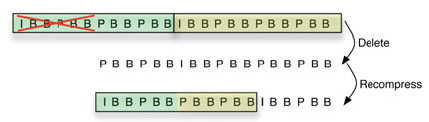
\includegraphics[width=10cm,height=10cm,keepaspectratio]{figuras/doble-compresion.png}
\end{center}
\caption{Reestructuración de GOP tras doble compresión, \cite{bestagini:2012}}
\label{fig_doble-compresion}
\end{figure}

\section{Identificación de la fuente}
La identificación de la fuente de adquisición es de vital importancia para muchos procesos judiciales, podría compararse con las pruebas balísticas para identificar un arma. Es por esto por lo que la identificación de la fuente en imágenes ha sido ampliamente estudiado por académicos en los últimos a\~nos con buenos resultados. 
Esta sección se restringe a la identificación de la fuente entendido como la identificación del modelo fuente en dispositivos móviles y no engloba otras temáticas como podría ser distinguir entre gráficos generados por ordenador o capturados. 

Existen muchas menos investigaciones sobre esta materia en video que en lo referente a imagen, a pesar de que un video se descompone como una secuencia de frames. Sin embargo, la menor resolución en video frente a imagen y las altas compresiones que se utilizan hacen que se pierde mucha información sobre la huella. \\

En \cite{naveen:2016} extraen una serie de fotogramas del video en base a la luminosidad para extraer el PRNU mediante la descomposición \textit{wavelet} de Daubechies de cuarto nivel a los que se aplica el filtro de Wiener. Se computa la correlación entre el ruido de cada frame para posteriormente evaluarlo mediante PCE (del inglés \textit{Peak-to-Correlation Energy}). Se utiliza un método de clasificación en el que las imágenes a analizar son caracterizadas en uno u otro grupo según el PCE. \\

En \cite{chen:2007} tratan el video como una secuencia de $N$ frames, para cada uno de esos frames extraen el PRNU y utilizan el estimador de máxima verosimilitud para identificar el PRNU del video. Para decidir si dos videos fueron tomados por la misma cámara se basan en la covarianza normalizada y en el PCE: si provienen del mismo dispositivo entonces el PCE es grande por el pico en la covarianza normalizada y en caso de no provenir de la misma fuente la covarianza normalizada parecerá ruido blanco. En las pruebas se utilizaron $25$ cámaras y muestra como el nivel de compresión del video es crucial para el algoritmo, cuanta mayor compresión menor calidad y más tiempo de video (en algunos casos $10$ minutos de video) se necesita para obtener un PRNU suficientemente bueno, lo que hace que este método no sea efectivo para videos de corta duración grabados por móvil. \\ 

En \cite{yahaya:2012} utilizan un subconjunto de los coeficientes AC de la transformada DCT formado a partir de tres índices $p$, $q$ y $r$ que toman $8$ orientaciones diferentes. Para cada una de esas orientaciones se calculan $9$ estadísticos en base a la relación de orden entre $p$ y $q$ y entre $r$ y $q$ lo que da un total de $72$ estadísticos diferentes que denominan caracerísticas CP, también utilizados en otros trabajos de estegoanálisis, que utilizarán como \textit{input} para un clasificador de tipo SVM. Para las pruebas utilizan $4$ modelos de cámara diferentes y $10$ videos de cada una de ellas, obteniendo una precisión del $100\%$. \\

En \cite{dong:2010} utilizan características propias de la codificación MPEG-2, características relacionadas con la tasa de bits, los factores de cuantificación y los vectores de movimiento. Tanto la tasa de bits como los factores de cuantificación y los vectores de movimiento no son parámetros fijos en el estándar MPEG-2, cada fabricante establece unos en concreto según el sensor. Tras extraer estas características, se utiliza un clasificador SVM entrenado. Para las pruebas utilizan videos de ocho codificadores distintos y obtienen precsiones por encima del $86\%$. Hay que tener en cuenta que videos obtenidos de cámaras que compartan el mismo codificador de MPEG-2 no serán clasificados como distintos por lo que este método solamente sirve para garantizar que dos videos provienen de distinta fuente. \\

En \cite{gprnu:2016} se basan en que dentro de los canales RGB el verde es el que tiene más información sobre la huella. Por ello extraen el canal verde de la imagen y mediante interpolación bilineal redimensionan los frames a tama\~no $512$x$512$ a los que extraen el ruido mediante \textit{soft-thresholding}. El PRNU del video lo obtienen como la media de los ruidos de cada frame y los clasifican utilizando la correlación como medida de similitud. En las pruebas se muestra cómo los resultados de este proceso con el G-PRNU (\textit{Green PRNU}) son mejores que con el PRNU. \\
